\documentclass{article}
 
\title{Intro to DIY Off Grid Systems}
\author{Demand for Energy Equality}
\date{October 2017 \\ Root source version: Version 2.0 \\ Translation version: Version 0.1}

%inherited code
\usepackage{amsmath,amsthm,amssymb,epsfig}
\usepackage{hyperref}

% imports for images
\usepackage{caption}
% \usepackage[demo]{graphicx}
\usepackage{graphicx}
% \usepackage{float}

% import for resuming enumerated list
\usepackage{enumitem}

% colour import
\usepackage[dvipsnames]{xcolor}

% code to remove numbering but keep the contents page filled
\setcounter{secnumdepth}{0}

\theoremstyle{definition}
\newtheorem{thm}{Theorem}[section]
\newtheorem{lem}[thm]{Lemma}
\newtheorem{prop}[thm]{Proposition}
\newtheorem{cor}[thm]{Corollary}
\newenvironment{pf}{{\noindent\sc Proof. }}{\qed}

\theoremstyle{definition}
\newtheorem*{defn}{Definition}
\newtheorem*{exmp}{Example}
\newtheorem*{prob}{Problem}
\newtheorem*{info}{Information}
\newtheorem*{warn}{Warning}
\newtheorem*{quest}{Question}
\newtheorem*{blockq}{Block Quote}
\newtheorem*{strong}{Strong}
\newtheorem*{code}{Code}
\newtheorem*{coderesult}{Code Result}

\theoremstyle{remark}
\newtheorem*{rem}{Remark}
\newtheorem*{note}{Note}
\newtheorem*{exer}{Exercise}

\setlength{\oddsidemargin}{0.25 in}
\setlength{\evensidemargin}{-0.25 in}
\setlength{\topmargin}{-0.6 in}
\setlength{\textwidth}{6.5 in}
\setlength{\textheight}{8.5 in}
\setlength{\headsep}{0.75 in}
\setlength{\parindent}{0 in}
\setlength{\parskip}{0.1 in}

\hypersetup{
    colorlinks=true,
    linkcolor=black,
    urlcolor=NavyBlue,
    pdfborderstyle={/S/U/W 1}
}

%%%%%%%
% Some commonly used notation
%%%%%%%

\def\R{{\mathbb R}}
\def\X{{\mathcal X}}
\def\Y{{\mathcal Y}}
\def\E{{\mathbb E}}
\def\sign{{\rm sign}}

% END inherited code

\begin{document}
 
\maketitle{}

\begin{center}
  
\includegraphics[width=0.25\paperwidth]{../Images/image_0_0_(demand_energy_equality).png}
\end{center}

\begin{center}
  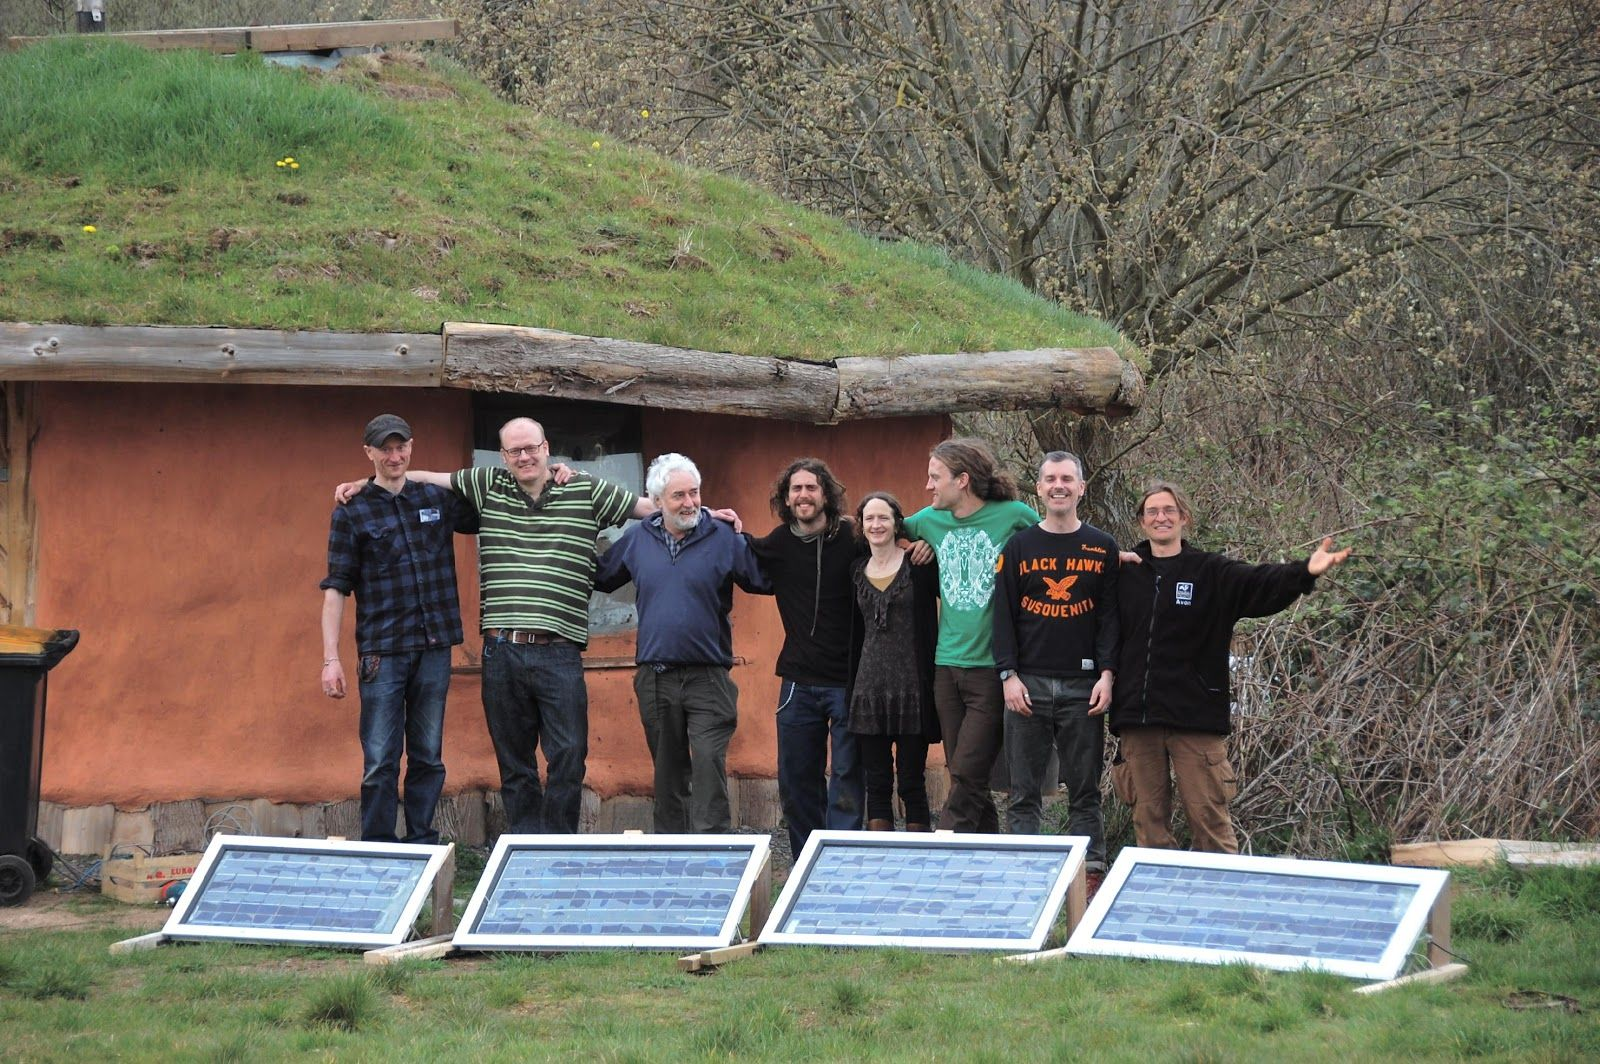
\includegraphics[width=0.65\paperwidth]{../Images/image_0_1_(off_grid).png}
\end{center}

\vfill
  

\includegraphics[]{../Images/image_0_2_(license).png} \newline
This guide is provided under a \href{https://creativecommons.org/licenses/by-sa/4.0/legalcode}{\underline{Creative Commons BY-SA}} license: \newline
Material may be freely shared and adapted under the following terms: You must give appropriate credit, provide a link to the license, and indicate if changes were made, and further distribution must be under the same license as the original.

\newpage

\tableofcontents

\newpage

{\color{blue}\section{Preface}} % (fold)
\label{sec:preface}

  {\color{blue}\subsection*{Introduction}} % (fold)
  \label{sub:introduction}
  
    This PDF has taken the content of the \href{https://www.demandenergyequality.org/get-started-with-offgrid}{\underline{"Intro to DIY Off Grid Systems"}} PDF and put them into a form which can be easily corrected, improved and translated by the community using LaTeX a markdown language for technical topics.

  % subsection introduction (end)

  {\color{blue}\subsection*{Notes}} % (fold)
  \label{sub:notes}

    Please note the modifications which have been made \& where you can find updates.

    \begin{enumerate}
      \item All the content of the PDF and put them into a form which can be easily corrected, improved and translated by the community using LaTeX a markdown language for technical topics.
      \item Any updates, corrections or translations to the PDF will be available at \href{https://github.com/darigovresearch/Intro-to-DIY-Off-Grid-Systems}{\underline{https://github.com/darigovresearch/Intro-to-DIY-Off-Grid-Systems}} so do return periodically to check if you have the latest version.
      \item Modifications from the original work includes typo correction, card merging \& consistency consolidation (see the commit history for [en] for the specific changes if any).
    \end{enumerate}

    Feel free to share the PDFs and give the repository a star so more people are likely to see this work and can get the most out of it.

  % subsection notes (end)

  {\color{blue}\subsection*{License}} % (fold)
  \label{sub:license}

    Unless otherwise specified, everything in this PDF is covered by the following licence:

    
\includegraphics[]{../Images/image_0_2_(license).png} \newline

    This work was based on the work \textbf{\textit{Intro to DIY Off Grid Systems}} by \href{https://www.demandenergyequality.org/}{\underline{Demand Energy Equality}}, licensed under a \href{https://creativecommons.org/licenses/by-sa/4.0/legalcode}{\underline{Creative Commons BY-SA}}.

    To see this work in full go to \href{https://www.demandenergyequality.org/get-started-with-offgrid}{\underline{https://www.demandenergyequality.org/get-started-with-offgrid}}
  
  % subsection license (end)

% section preface (end)

\newpage

{\color{blue}\section{Introduction}} % (fold)
\label{sec:introduction}

  {\color{blue}\subsection{The Demand Energy Equality project}} % (fold)
  \label{sub:the_demand_energy_equality_project}

    Demand Energy Equality (DEE) is a UK based community energy project that seeks to provide practical energy education, relating mainly to solar generation. We are a group working for systemic change in the way energy is produced, distributed, controlled, delivered and used. These aims are within the context of rising energy inequality (in the UK, at least), rising fuel bills, climate change and the increasing cost of fossil fuel extraction. See our website to find out more about the project.

    Through teaching people hands-on energy skills we also aim to develop their relationship with energy, and enable them to understand it better: where it comes from, how it is used and how it relates to their demand and needs. Ultimately we aim for this to change behaviour, leading to better use of energy and overall reduced demand. Reduced energy use is an unavoidable fact of the relatively near future – far better to prepare now than be surprised later on.

  % subsection the_demand_energy_equality_project (end)
  
  {\color{blue}\subsection{Using this guide}} % (fold)
  \label{sub:using_this_guide}

    This written guide is for anyone interested in building their own basic off grid energy system, or learning more about the concepts involved. It assumes no prior knowledge of any kind relevant to completing a fully working project. The guide is designed to to act as a learning aid for participants on the ‘Introduction to Off Grid’ workshops run by Demand Energy Equality, and can be used alongside other DIY guides and resources provided by DEE. 

    The guide provides a summary of the concepts involved in energy systems, gives descriptions of some of the more common components used to build off-grid solar installations, and shows how to carry out the basic energy modelling needed to correctly size a system. Links to useful sources of further research are included at the end of the guide.

    This particular version reflects the most recent iteration of the design of off grid systems as practiced by DEE, but it is likely that it may evolve and expand over time.  Because we occasionally review and update our content, the guide may not always be in line with the other DIY resources published by DEE, and may not exactly reflect the format of current workshops. Contact DEE if you need an update on any recent changes. 

    You will find the latest version of this guide available to download from the DEE website, as and when this guide is updated, alongside our \href{https://www.demandenergyequality.org/resources/}{\underline{other guides and resources}}.

    For a chance to gain practical experience of the material covered in this guide, please take a look at the workshops offered on the DEE website (\href{www.demandenergyequality.org}{\underline{www.demandenergyequality.org)}}.

    We encourage you to share the skills you learn with others through your own workshops, particularly if you are able to target and work with low-income communities. Please contact us for any support you feel you may need if you plan to do this.

  % subsection using_this_guide (end)

  {\color{blue}\subsection{Disclaimer}} % (fold)
  \label{sub:disclaimer}

    This guide is for general guidance only and whilst every effort is made to ensure that the information it contains is correct, it should not be relied upon as accurate. The information / advice contained within this guide is intended for use within the UK only and by persons of no less than 18 years of age. Use this guide at your own risk.

    DEE will not accept any liability for any loss, damage, injury or negligence direct or indirect from use of the information / advice contained within this guide.

  % subsection disclaimer (end)

  \newpage  

% section introduction (end)

{\color{blue}\section{Basic concepts}} % (fold)
\label{sec:basic_concepts}

  {\color{blue}\subsection{Power consumption}} % (fold)
  \label{sub:power_consumption}

    \textit{Power} is a measure of  work done in any instant, measured in watts (W). You'll typically find a value of the number of watts an appliance needs to operate written on the outer case or on the adaptor that plugs into the wall socket. The power consumption of a laptop, for example, is commonly around 60 watts (less for basic netbooks and more for high-end laptops with advanced graphics). This is the measurement that tells you how much power you actually need to deliver for every moment that the appliance is in operation. As it is an instantaneous measure you can find a more useful measure by introducing time into the equation. The unit we will use for this is watt hours (Wh), which is a measurement of energy. Energy is directly related to power and time using the equation:

    \begin{equation}
      \text{Energy} (Wh) = \text{Power} (W) \times \text{Time} (h)
    \end{equation}

    In this way we can compare the energy used by a kettle that runs at about 3000W for 6 mins at a time with a laptop running at 60W for 3 hours at a time. The energy required for a single kettle boil is therefore: 3000W $\times$ 0.1 hours = 300Wh. The energy required for three hours of laptop use is: 60W $\times$ 3 hours = 180Wh. 
  
  % subsection power_consumption (end)

  {\color{blue}\subsection{Voltage}} % (fold)
  \label{sub:voltage}

    \textit{Voltage} is the potential  to do work. It is measured in volts (V). Imagining electricity like a flow of water turning a water wheel, the voltage is like the height of the flow of water flowing into the water wheel. If the voltage is too low the water will just flow underneath the water wheel and the water wheel won't turn. A higher voltage will turn the wheel effectively. A voltage too high could be damaging to the water wheel. In the same way a voltage too high for an appliance will damage the appliance. 

  % subsection voltage (end)

  {\color{blue}\subsection{Current}} % (fold)
  \label{sub:current}

    \textit{Current} is the flow of electricity and is measured in amps (A). Using the same flow of water analogy current is the amount of water flowing. Lots of flow allows the water wheel to turn faster, less flow allows it to flow less quickly. Power is directly related to voltage and current using the equation:

    \begin{equation}
      \text{Power} (W) = \text{Voltage} (V) \times \text{Current} (A)
    \end{equation}
    
    Essentially what this means is that the amount of power available increases if either the volts or the amps increase, or of course if both increase. Similarly, the amount of power available decreases if either the volts or the amps decrease, or if both decrease.

  % subsection current (end)

  {\color{blue}\subsection{Resistance}} % (fold)
  \label{sub:resistance}

    \textit{Resistance} reduces the flow of electricity through a wire or component. It is a bit like forcing the water from our analogy to travel through a gorge filled with rapids. Relative to the same amount of water flowing through a smooth channel, the ability to deliver power at the other end will be reduced. All components and wires have an internal resistance that uses up the power you are supplying without doing any useful work. This is something we want to minimise in our systems. 
  
  % subsection resistance (end)

  {\color{blue}\subsection{Series and parallel circuits}} % (fold)
  \label{sub:series_and_parallel_circuits}

    Electrical circuits behave in different ways depending on how they are connected. There are two types of connections: 

      \begin{table}[!ht]
        \centering
        \begin{tabular}{|| c | c | c | c ||}
          \hline
          \multicolumn{2}{|c|}{Series Circuits}  & \multicolumn{2}{|c|}{Parallel Circuits}  \\
          \hline \hline
          Connect & $+ \rightarrow -$ & Connect & $+ \rightarrow +$ \\
          \hline
          Connect & $- \rightarrow +$ & Connect & $- \rightarrow -$ \\
          \hline
        \end{tabular}
        \label{table:two_types_of_connections}
      \end{table}

    Intro series connections the voltage will be shared across two components while the current will be constant along the components connected. In terms of power sources (like panels and batteries) this means that the voltage will sum across the panels connected in series while the current will stay constant. 

    For power consumers (like appliances) connected in series, the total voltage from the power source will be shared between each appliance. For example, two identical 6V bulbs in series connected to a 12V battery will light up as expected, since each bulb will receive 12 \(\div\) 2 volts. The current to each bulb will be constant, which is fine as that is what the bulbs require. Two 12V bulbs connected in series to a 12V battery will not light up properly. You may see a dim glow but as the voltage each bulb is receiving is only 6V this is not enough to properly light the bulbs. In parallel connections the voltage will be constant across the appliances and the current will be shared.

    In terms of power sources (like panels and batteries) this means that the voltage will be constant across the appliances and the current will sum. For power consumers (like appliances) connected in parallel, each appliance will have the full voltage available to it and each will share the total current drawn. So two 12V bulbs in parallel with a 12V battery will light up with a current draw equal to the sum of the two bulbs. Two 6V bulbs in parallel with a 12V battery will more than likely break as each will have 12V supplied to it, double what it requires. 
  
  % subsection series_and_parallel_circuits (end)

% section basic_concepts (end)

{\color{blue}\section{What is an off grid system}} % (fold)
\label{sec:what_is_an_off_grid_system}

  Off grid renewable systems refer to systems that have no connection to a wider electrical grid, that generate their power from renewable sources. In the UK, the grid in this definition would be the National Grid, which distributes electrical power from large power stations to consumers through a series of power transmission cables.

  There are three main elements of an off grid renewable energy system: generation, storage and consumption. Generation covers the part of the system that converts a renewable energy source into useful electrical energy, storage covers the means by which that energy is stored for use when needed, and consumption covers the appliances and equipment that draw power from the system to do the work we want them to do.

  We also need to consider system controls that the system to be monitored and regulated. These are used to make sure that too much stress is not placed on any part of the system when it is in use, to keep it in good working order.

  \begin{center}
    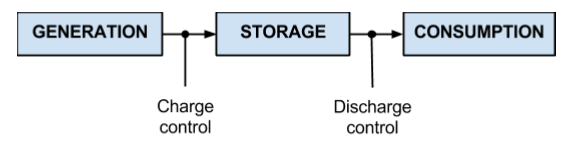
\includegraphics[width=0.60\paperwidth]{Images/image_3_1_(off_grid_diagram).png}
  \end{center}

  {\color{blue}\subsection{Why 12 Volt}} % (fold)
  \label{sub:why_12_volt}

    Both the solar panels and the off grid systems recommended by Demand Energy Equality are based around 12 Volt (12V) systems. This is because 12V is a standard off-grid electrical voltage. Designing around a voltage of 12V makes a lot of technology and equipment available at relatively low cost, meaning systems are simple to design, build and maintain. 12V is the voltage of car electrical systems, so anything that plugs into a car cigarette lighter socket should be compatible with our systems. Lights, music systems, phone and laptop chargers, even kettles, fridges and cookers are readily available at 12V. 

    Another reason to choose 12V is that it is a relatively safe voltage to work at. Electricity can be dangerous at any voltage but a low voltage system will not cause an electric shock. There are some safety points to consider, that will be mentioned in the sections of this guide titled 'Safety Note'.

  % subsection why_12_volt (end)

% section what_is_an_off_grid_system (end)

{\color{blue}\section{Generation}} % (fold)
\label{sec:generation}

  This guide primarily focuses on solar installations but for completeness other forms of popular small scale renewable energy generation are referred to in this section. Not all information in this guide is relevant to all forms of electrical generation so be sure to consult other resources when working with anything other than small scale solar.

  When charging batteries, the voltage of the power supply must be higher than the nominal voltage of the battery. Most batteries need to be charged at a very specific voltage, so make sure that your generation voltage is in the correct range. 

  {\color{blue}\subsection{Solar panels}} % (fold)
  \label{sub:solar_panels}

    Solar panels generate energy by utilising the energy from photons from the sun to excite electrons in a silicon semiconductor creating a voltage difference. The open circuit voltage (Voc) of a solar array used in a 12V system with lead acid batteries is generally around 18V. 

    DEE offer one day workshops and online resources to teach people how to build their own solar panels from low cost and reused materials. Find out more on the \href{http://www.demandenergyequality.org/}{\underline{DEE website}}.

    For more information on how solar cells work see Resource 6.
    
    \begin{center}
      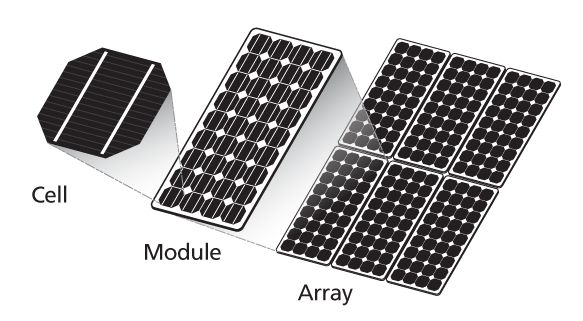
\includegraphics[width=0.45\paperwidth]{Images/image_4_1_(solar_breakdown).png}
    \end{center}
  
  % subsection solar_panels (end)

  {\color{blue}\subsection{Wind turbines}} % (fold)
  \label{sub:wind_turbines}

    Wind turbines utilise the wind to power a generator. Inside the generator the wind turns a magnet across a conductor (such as coils of copper wire), creating a current in a circuit. Wind turbines can be made from recycled materials. There are lots of instructions available online and different organisations offer courses in the UK. Communities such as Grow Heathrow have made their own wind turbines from free and recycled materials.

    See Resource 7 for more information.
  
  % subsection wind_turbines (end)

  {\color{blue}\subsection{Hydro-generation}} % (fold)
  \label{sub:hydro_generation}

    Similar to wind turbine generation, hydro-generation utilise a flow of water to power a generator. Inside the generator the water turns a magnet across a conductor (such as coils of copper wire), creating a current in a circuit. Small scale hydro generators can be made from recycled materials, and can convert the energy contained in hillside streams. Again, instructions can be found online. The community Steward Wood has made a hydro-generator from recycled materials, and more information can be found in Resource 8.
  
  % subsection hydro_generation (end)

  {\color{blue}\subsection{Cycle powered generation}} % (fold)
  \label{sub:cycle_powered_generation}

    Cycle powered generation works, again, in a similar way to wind and hydro. Cycle powered generators can be easily constructed from electric DC motors. Direct drive motors that usually spin when a voltage is applied to them will also generate a voltage when spun. If you use motors with the right torque and revolution ratio they can be an ideal match up to a person cycling at a steady pace.

    Cycle generators make a good supplemental power system in winter when solar production declines.

    See Resource 9 for more information.
  
  % subsection cycle_powered_generation (end)

% section generation (end)

{\color{blue}\section{Storage}} % (fold)
\label{sec:storage}

  {\color{blue}\subsection{Batteries}} % (fold)
  \label{sub:batteries}

    Batteries are the heart of our system, and we will essentially design our whole system around them. The function of the batteries is to store electrical energy for use later on. This is what will make our solar panels actually useful, as we can take the power produced by the panels and use it in faster bursts when we want it, or when the sun has gone down. 

    This guide focuses on 12V batteries and systems but there is no reason you could not use 6V batteries (2 in series makes a 12V battery) or even design a solar panel to charge AA or AAA rechargeable batteries (1.2V each). The principles are the same. 

    If you have multiple 12V batteries you can use them in the same 12V system by connecting them in parallel. In this case the voltage will stay at 12V and the capacity of the battery bank (measured in Amp hours (Ah)) will increase. 
  
    \subsubsection{Specifications} % (fold)
    \label{ssub:specifications}

      Labels on batteries will indicate the most important bits we need to know: the voltage of the battery and the capacity of the battery. The capacity of the battery is measured in Amp Hours (Ah). This gives an indication of the capacity of the battery over time. In theory a 60Ah battery could run at 1A for 60 hours or 6A for 10 hours, although increasing the load being drawn will generally decrease the available capacity of the battery. Most battery capacities are given for a 20 hour discharge rate (C20), meaning that a battery will deliver its rated capacity only when the current being drawn is enough to discharge the battery in 20 hours. For example, a 60Ah battery can supply 3A of current for 20 hours, but if the current is increased to 6A, the battery will be fully discharged in less than 10 hours.

      Batteries also have a limit to the flow of current they can deliver. As you draw a higher current the voltage of the battery will drop due to the internal resistance of the battery. For the applications detailed in this guide this will not be relevant, but check your battery specifications if you do require high current.
    
    % subsubsection specifications (end)

    \subsubsection{Battery types} % (fold)
    \label{ssub:battery_types}

      \begin{itemize}[label={}]
        \item \textbf{Nickle Cadium (NiCd)} and \textbf{Nickel Metal Hydride (NiMH) -} These are common in small rechargeable batteries, coming in AA, AAA, C, D, 9V etc. They are also used in older cordless power tool batteries. Nickel-based batteries suffer from the ‘memory effect’, meaning that they gradually lose their maximum energy capacity if they are repeatedly recharged after being only partially discharged

        \item \textbf{Lithium Iron (Li-ion) -} This is the kind of battery used in mobile phones, laptops, rechargeable torches, cordless power tools and electric vehicles. For their size and weight they are high capacity, but expensive and generally less reliable second hand. 

        \item \textbf{Lead-Acid -} These are the most common 12V batteries and the ones we focus on in this guide. They are easy to come by, suitable for off-grid systems and easy to test and buy second hand. Some lead-acid batteries can release flammable gases when used and therefore should be used in a well ventilated space. Lead-acid batteries come in several different types, with very different properties, so it’s important to understand the differences. 
      \end{itemize}

      Differences in construction:

      \begin{itemize}[label={}]
        \item \textbf{Absorbed glass mat (AGM)} batteries have a glass fibre mat soaked in electrolyte to separate the cells. This mat greatly reduces gassing, allowing them to be completely sealed, which makes them useful in portable devices and similar roles. Gas build-up remains a problem when the battery is deeply or rapidly charged or discharged, so AGM batteries include a one-way blow-off valve, and are often known as "valve regulated lead–acid", or VRLA, designs.

        \item \textbf{Gel} batteries contain a gel coating around the battery plates to stop gases escaping. As with AGM batteries, they can be completely sealed. Gel batteries are particularly suited to slow charging and discharging, making them suitable for renewable systems.

        \item \textbf{Flooded} (or vented) batteries are not sealed, and have ventilation caps on each cell. These batteries emit hydrogen gas when being charged, and need to be stored in a well ventilated space. Over time, the level of electrolyte in the battery will drop, and they need topping up with distilled water every few weeks.
      \end{itemize}

      Differences in function:

      \begin{itemize}[label={}]
        \item \textbf{Car} or \textbf{Starter} batteries have an internal structure designed to deliver a high current for a short time and then be recharged directly after. This is unsuitable for off-grid use, as we want to utilise the power over a longer period at a slower rate. Car batteries will power a 12V system but will quickly wear out with regular charging and discharging so unless you are getting them for free or for very low cost it is not worth bothering with them.

        \item \textbf{Leisure} or \textbf{Marine} batteries are designed to be used in boats, campervans and caravans where they can serve the dual function of starting an engine and powering electrical appliances. They can be discharged deeper than car batteries, but will generally only serve moderate use as an auxiliary power source when the engine is not running or when there is no grid hook-up available. They will not endure as many discharge cycles as a dedicated deep cycle battery.

        \item \textbf{Deep cycle} batteries are designed to be discharged as much as 75\% before being charged again, and deliver a lower current over a longer period of time. They can be AGM, Gel or Flooded, but will be made from heavier, thicker lead plates than other batteries, which makes them better able to endure repeated deep discharge cycles. Deep cycle batteries can be used in uninterruptable power supply (UPS) systems, or to provide traction power for golf buggies and forklift trucks, or to provide power to industrial equipment at remote sites. There are also deep cycle batteries made specifically for off grid renewable energy applications. 
      \end{itemize}
    
    % subsubsection battery_types (end)

    \subsubsection{How lead acid batteries work} % (fold)
    \label{ssub:how_lead_acid_batteries_work}

      12V Lead Acid batteries contain 6 cells, each of 2V, connected in series internal to the battery. Each cell consists of two lead plates surrounded by a sulphuric acid electrolyte. The transfer of ions between the lead and the acid when the battery is charged are what allow it to store electrical energy.

      During the charging process electrons are forced from the positively charged plate back to the negatively charged plate. This charge is then held and stored until a draw is required, at which time the electrons flow from the negative plate through an electrical circuit to the positively charged plate. The chemical reaction that takes place during this process causes a build up of sulphur crystals to develop on the lead plates, which is called ‘sulfation’. 

      The normal voltage range of a 12V battery is between 10.5 and 12.7V. Measuring the voltage of a battery allows you to determine its State of Charge (S.o.C.). A battery with a voltage of 12.7V has a S.o.C. of 100\%, and a battery with a voltage of 10.5V has a S.o.C. of 0\%. If the S.o.C. is kept above 50\% (measured at 12V) most of the build up of sulphur crystals during discharging readily dissolves back into the electrolyte solution during charging. Over time, repeated sulfation plays a role in the reduction of battery efficiency over time. If the battery is over discharged this build-up can harden and become difficult or impossible to remove, permanently reducing the effectiveness of your battery. 

      \begin{center}
        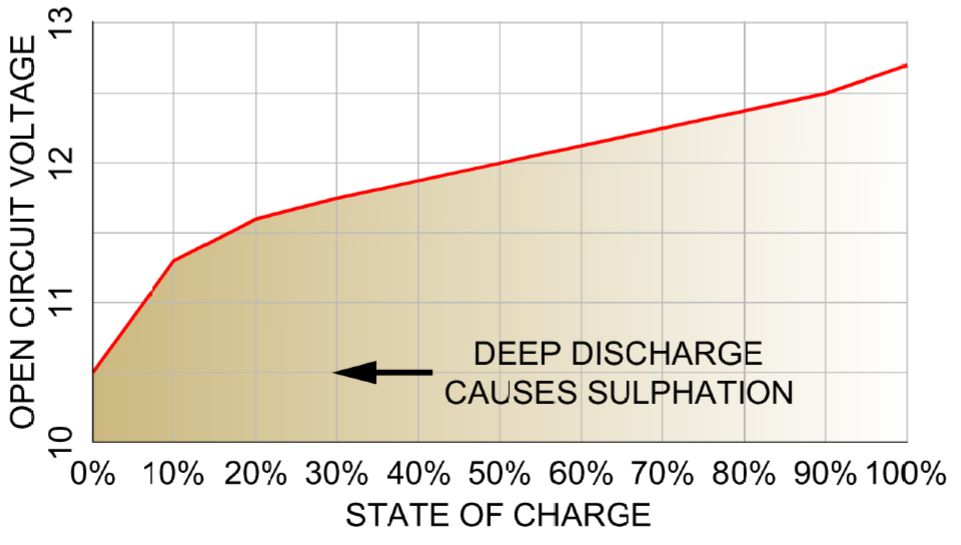
\includegraphics[width=0.65\paperwidth]{Images/image_5_1_(sulphation).png}
      \end{center}

      For more details on how lead acid batteries work see Resource 1
    
    % subsubsection how_lead_acid_batteries_work (end)

    \subsubsection{Carbon intensity} % (fold)
    \label{ssub:carbon_intensity}

      Carbon intensity is a standard measure of average carbon emissions for an activity or item. In the off-grid systems we design we aim to be much less carbon intensive than the national grid which currently releases between 350g and 400g CO2 per KWh of power supplied. Lead acid batteries, if used for their entire life-cycle of approximately 10 years have a carbon intensity of approximately 180g CO2 per KWh of power supplied. This obviously increases if you decrease the life span of your batteries. If you use your battery for only one year before its end of life the carbon intensity increases 10 fold making the off-grid system over four times more carbon intensive than the national grid. For this reason we do everything we can to optimise the life-span of the batteries, and this influences many of the decisions we make in designing our system. Using second hand batteries is one way reduce the impact of your system, particularly if you can tap into a waste stream. 
    
    % subsubsection carbon_intensity (end)

    \subsubsection{Buying second hand batteries} % (fold)
    \label{ssub:buying_second_hand_batteries}

      When buying second hand batteries you need to ensure you don't spend money on a dud battery. Dud batteries can show a full S.o.C, but may not be able to hold the charge over time or supply anything more than a minimal load. Two ways to test are:

        \begin{itemize}
          \item Using a multimeter to ensure the battery is within the optimal voltage range. If a battery reads under 12V then it is likely not at its best. If it reads under 10.5V then it is definitely a dud and not worth taking. 
          \item Using a load tester to ensure the battery can deliver under load. This is a better test than using a multimeter, and will give you more information as to the ability of the battery to deliver over a high load. However, load testers are built for car batteries, meaning they'll give a conservative reading on a deep cycle battery.
          \item Carry out a discharge test. First make sure the battery is 100\% charged, and has been left to stabilise for a few hours. Then connect a load roughly the size of the 20 hour discharge capacity of the battery (e.g. if the battery is rated at 60Ah, connect a load that draws around 3 amps). After a number of hours (e.g. 4), disconnect the load, then leave the battery to stabilise for another couple of hours. Measure the voltage on the battery, and refer to the manufacturer’s specifications to calculate its new S.o.C (e.g. a reading of 12.3V will indicate it has been discharged around 25\%). The capacity of the battery will be Current \(\times\) Time \(\div\) discharge level (e.g. 3A \(\times\) 4 hours \(\div\) 0.25 = 48Ah).
        \end{itemize}
    
    % subsubsection buying_second_hand_batteries (end)

    \subsubsection{Caring for lead acid batteries} % (fold)
    \label{ssub:caring_for_lead_acid_batteries}

      Most of the equipment discussed in the remainder of this guide is designed to help you take the best care of the lead-acid batteries. As a general rule, keeping lead-acid batteries above 12V (50\% S.o.C.) will help ensure they keep functioning well. When moving lead-acid batteries aim to keep them level and upright to ensure the electrolyte solution does not flow between cells to become uneven.

      Even within this voltage range some sulfation will occur over time. You can mitigate this by following a charging routine that includes an ‘equalization’ charge cycle at least once a month. The charging voltage for lead acid batteries is usually between 13.5V and 13.8V, but to keep the electrolyte well-mixed, and to break up heavy sulfation, a higher equalization voltage of around 15V should be regularly applied. Most battery chargers will do this automatically. 

    % subsubsection caring_for_lead_acid_batteries (end)

  % subsection batteries (end)

% section storage (end)


{\color{blue}\section{Charge control}} % (fold)
\label{sec:charge_control}

  Charge controllers play a number of essential roles in ensuring that the correct charge is delivered to the battery at the correct time, protecting your batteries and increasing their life by: 

  \begin{enumerate}
    \item Optimising the input voltage to the correct level for the battery. Solar panels will output a higher voltage than the battery requires by design. The charge controller will regulate this voltage by detecting from the battery the optimal voltage to charge with, increasing as the battery charges. 
    \item Stopping charging when the battery is full. This will prevent damage to the battery through overcharging. 
    \item Stopping the panel from draining the battery at night. At night the battery will have a higher charge than the panel and hence the battery can send a current through the panel if directly connected. 
  \end{enumerate}

  \begin{center}
    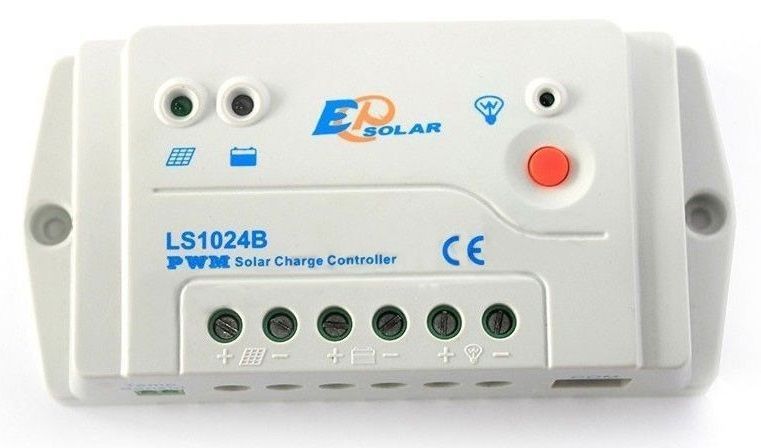
\includegraphics[width=0.25\paperwidth]{../Images/image_6_1_(charge_controller).png}
  \end{center}

  {\color{blue}\subsection{PWM and MPPT}} % (fold)
  \label{sub:pwm_and_mppt}

    \textbf{PWM} (Pulse Width Modulation) controllers regulate the voltage coming from a solar panel by rapidly switching the connection between the solar panels and the battery on and off. Since this doesn’t change the current, there is a loss in power reaching the battery. If using a PWM charge controller, the voltage of the solar array used should have an open circuit voltage of 17-18V in order to generate the voltages needed with minimal power lost. The overall power efficiency of PWM charge controllers is around 70-80\%.

    \textbf{MPPT} (Maximum Power Point Tracker) charge controllers include a DC voltage converter that increases the current proportional to the reduction in voltage, so the power reaching the batteries is optimised. This results in an overall power efficiency of 95\% or more, meaning more charge to the batteries. You can also use MPPT charge controllers to connect solar arrays with higher voltages, allowing much more flexible set-ups. For more information about how MPPT charge controllers work see Resource 2.
  
  % subsection pwm_and_mppt (end)

  {\color{blue}\subsection{Choosing the right charge controller}} % (fold)
  \label{sub:choosing_the_right_charge_controller}

    The correct charge controller will match the demands of your panels and batteries. If you are connecting a large panel array you will need to ensure the charge controller can handle the nominal input voltage and current of your panels. Similarly if you are using a large battery bank at a higher voltage (24V or 48V) you will need to ensure the charge controller can handle this voltage. More expensive MPPTs will generally give you more options. For a small set up with a couple of panels and batteries the inexpensive PWM charge controllers will be adequate. 
  
  % subsection choosing_the_right_charge_controller (end)

% section charge_control (end)

{\color{blue}\section{Discharge control}} % (fold)
\label{sec:discharge_control}

  As well as making sure you don’t overcharge your battery, you need to make sure you don’t discharge it to the point where it suffers from permanent sulfation. For this, you need something in place to disconnect loads when the the S.o.C. drops below an acceptable limit. Systems without discharge control are vulnerable to over-discharge of the battery, which is the easiest way to cause permanent damage to the batteries.

  Most charge controllers will have terminals to connect a load. This allows you to connect lights, DC chargers and other appliances through the charge controller, which will provide some discharge control Basic charge controllers will have a fixed low-voltage disconnect that is set at 11V. This is below the 50\% S.o.C. recommended discharge limit, so if using this type of charge controller you may want to include additional protection. Basic charge controllers also generally don't reconnect the load until the batteries have been fully recharged. More advanced charge controllers have a programmable low-voltage disconnect and reconnect level, that can be set to 12V or whatever voltage is appropriate.

  For loads that are drawn directly from the battery, you will need separate discharge control. The simplest way to do this is to include a battery guard in the system to cut power supply when the battery voltage drops below a specified limit. 

  You should also include a voltage display that shows the voltage of the system or some other way of displaying the battery S.o.C., allowing it to be monitored by users so they can self-regulate consumption according to how much the batteries are charged.

  \begin{center}
    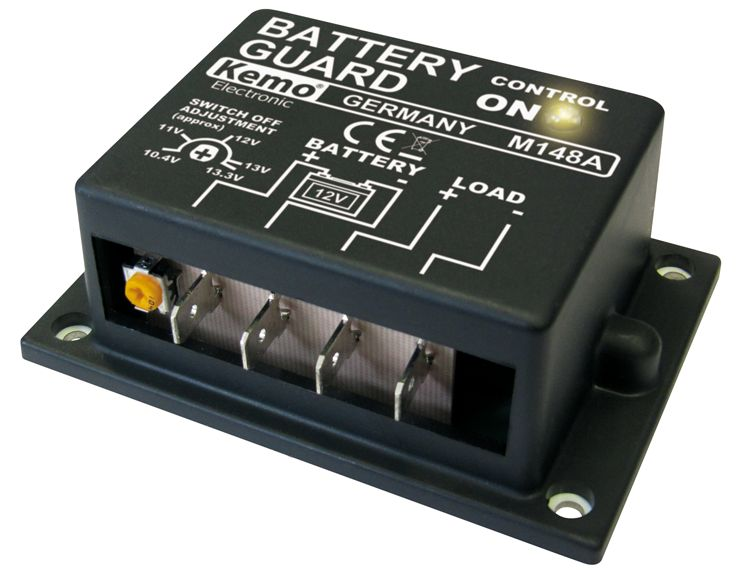
\includegraphics[width=0.15\paperwidth]{../Images/image_7_1_(discharge_control).png}
  \end{center}

% section discharge_control (end)

{\color{blue}\section{Other system level equipment}} % (fold)
\label{sec:other_system_level_equipment}

  {\color{blue}\subsection{Fuses}} % (fold)
  \label{sub:fuses}

    \begin{center}
      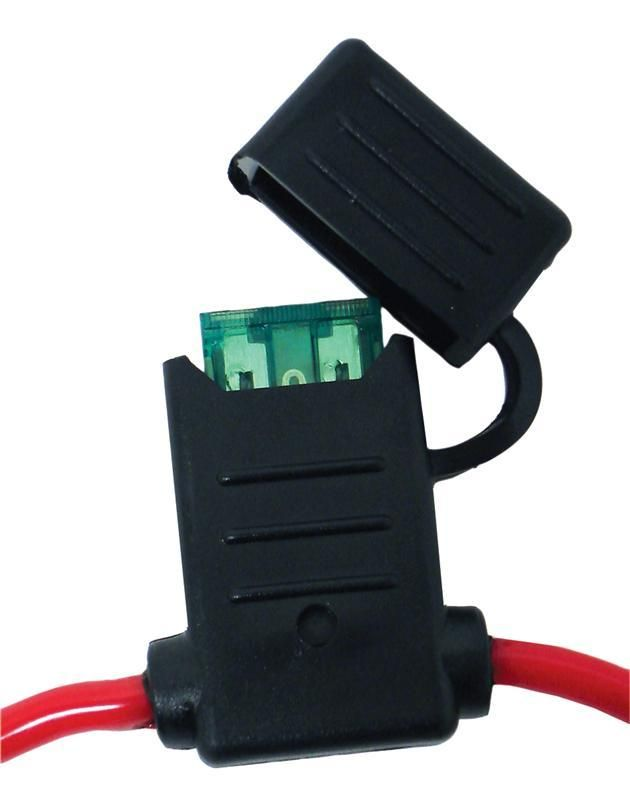
\includegraphics[width=0.15\paperwidth]{../Images/image_8_1_(fuse).png}
    \end{center}

    Fuses are a crucial part of any electrical system. A fuse is essentially just a thin piece of wire that will break when the current running through it is higher than the limit the wire can handle. This makes them ideal for protection against surges and short circuits, that if uninterrupted would present a fire risk, possibly damage your appliances and drain your batteries to empty. 
  
    \subsubsection{Size and placement} % (fold)
    \label{ssub:size_and_placement}

      Choose an appropriate fuse to handle slightly more than the highest expected current for the part of the system it is protecting. Fuses should be placed as close to the power source as possible, usually on the positive wire. If you install a fuse directly next to the battery the fuse will need to be able to handle the full current draw of every appliance. You can have multiple fuses protecting different parts of the system, i.e.. with a variety of different loads connected, each can have a separate fuse. With multiple fuses, you might find it useful to install them together in an easily accessible fuse box should they need to be replaced. 

      You can also use circuit breakers instead of fuses, which carry out the same function but can be reset instead of replaced.
    
    % subsubsection size_and_placement (end)

  % subsection fuses (end)

  {\color{blue}\subsection{Wire}} % (fold)
  \label{sub:wire}

    The thickness of the wire you use to transmit electricity is crucial for minimising line losses. Line losses occur due to the internal resistance of the wire used. The higher the current, the higher the potential line losses and the thicker the wire required. 

    Wire thickness is measured in cross-sectional area in square millimeters ($mm^{2}$), or American Wire Gauge (AWG). See Resource 3 for a handy calculator to help you gauge the thickness of wire required. 

    If you still aren't sure whether or not a given wire will be adequate you can test it out. Take the wire to the desired length and connect to your batteries and lights/appliance. Measure the voltage at the battery and again across the appliance. A lower voltage measurement across the appliance is caused by internal resistance in the wire. If the drop is significant (greater than 4\% of the battery voltage) consider using thicker wire. 
  
  % subsection wire (end)

  {\color{blue}\subsection{DC voltage conversion: Step Up and Step Down}} % (fold)
  \label{sub:dc_voltage_conversion_step_up_and_step_down}

    As described in the section above, internal resistance of conducting wire can mean you lose power in transmission if your wire is not thick enough. Thick wire is expensive, so if you need to transport your electricity long distances from your panels to where you will be using the electricity you will want to consider alternatives.

    Line losses occur based on the current transportation: the higher the current the higher the potential line losses. So converting to a higher voltage and a lower current will result in much lower line losses for the same wire thickness, allowing you to use thinner wire to transmit the same amount of power. 

    \textbf{Step Up} converters convert a power supply into a higher voltage with lower current. Installing a step up after the power source, before transmission will reduce the line losses in transmission.

    \textbf{Step Down} converters can take a higher voltage down to 12V, allowing you to connect 12V appliances as normal. These are useful when using a power source that has been stepped-up for transmission, or when connecting to a large 24V or 48V battery bank.

    \begin{center}
      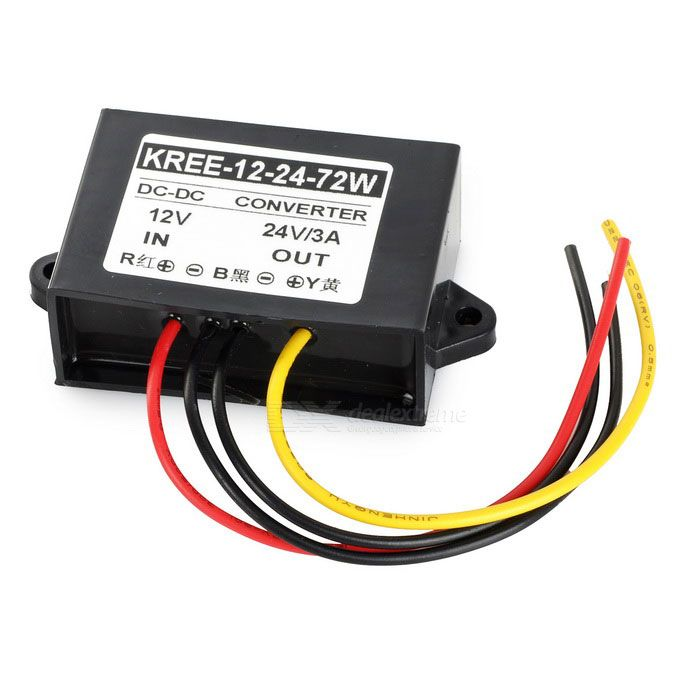
\includegraphics[width=0.15\paperwidth]{../Images/image_8_2_(dc_dc_converter).png}
    \end{center}

    TODO ADD BOX

    Safety Note
    
    In DC (direct current) systems higher voltages can become dangerous quickly. This is due to the constant voltage in DC. In AC (alternating current) systems the voltage fluctuates between positive and negative voltages meaning that many times each second the voltage drops to zero making it easier to release from the source of the electric current causing the shock. This does not happen in DC circuits. This is important if you choose to step up your voltage for transmission. Working at voltages higher than 48V DC can create very dangerous voltages and circuits and should only be done if you are confident and have taken stringent precautions to protect users from potential electric shock. For most small scale off grid purposes 12V is sufficient. 
  
  % subsection dc_voltage_conversion_step_up_and_step_down (end)

  {\color{blue}\subsection{Connectors}} % (fold)
  \label{sub:connectors}

    Connectors are basically just safe and secure ways to connect wires together. There are a vast range of connectors on the market and you may find ones not mentioned here suit your needs better. This section outlines the ones used in the Intro to Off Grid workshop. The simplest way of connecting together two wires is to twist them, solder them, then insulate them using heatshrink or electrical tape. This can also be the most secure if done correctly, but cannot be easily undone, so using the connectors listed below may be more convenient.

    TODO ADD BOX

    Safety Note
     
    Unsecured electrical connections can cause sparks which can lead to fires. This can be compounded by gases released by batteries. Securing and insulating connections can minimise this risk.
  
    \subsubsection{Terminal blocks} % (fold)
    \label{ssub:terminal_blocks}

      Terminal blocks are very useful for connecting together loose ends of wire. They are also useful in creating parallel connections, as you can have multiple wires in either end of the block. Another useful feature of connector blocks is that the screws that hold the wires into the blocks are conductive themselves, meaning you can apply a multimeter directly to them for testing.

      \begin{center}
        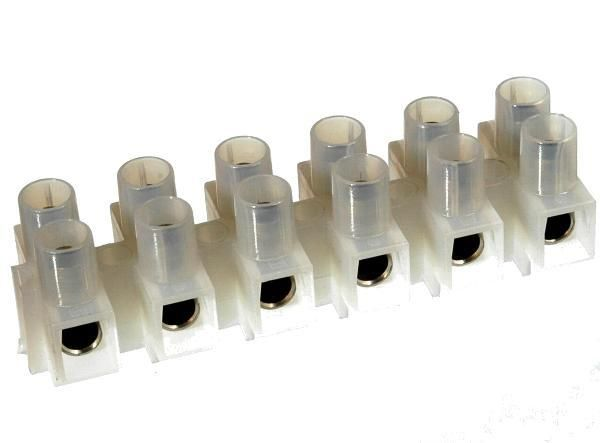
\includegraphics[width=0.15\paperwidth]{../Images/image_8_3_(terminal_connector).png}
      \end{center}

    % subsubsection terminal_blocks (end)

    \subsubsection{Crimp connectors} % (fold)
    \label{ssub:crimp_connectors}

      A wide variety of connector types can be crimped onto electrical wire to connect appliances in a low voltage system. A crimping tool is needed to attach these connectors to the wire. Crimp connectors come in three sizes, and these sizes relate to the thickness of the wire you are using, rather than the connectors themselves.

      TODO ADD BOX

      Red Connector  0.5-1.5mm 2  wire

      Blue Connector  1.5-2.5mm 2  wire

      Yellow Connector  2.5-6mm 2  wire

      \textbf{Spade connectors:} Many switches and components you are likely to use on small 12v systems will have a male spade connection on them. The easiest way to connect to these is with a female spade crimp connector.  
    
      \begin{center}
        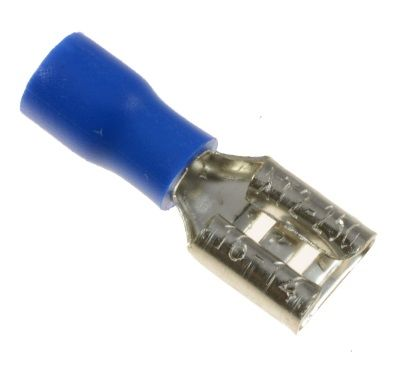
\includegraphics[width=0.15\paperwidth]{../Images/image_8_4_(spade_connector).png}
      \end{center}

      \textbf{Ring Connectors:} These are useful for connecting to batteries and high-current appliances that have bolts at the terminals. The rings fit around the bolts allowing the bolts to hold the wires safely in place. The rings come in a range of sizes to support the range of battery bolts you might encounter.
    
      \begin{center}
        
\includegraphics[width=0.15\paperwidth]{../Images/image_8_5_(ring_connector).png}
      \end{center}
    
    % subsubsection crimp_connectors (end)

  % subsection connectors (end)

% section other_system_level_equipment (end)

{\color{blue}\section{Usage level equipment}} % (fold)
\label{sec:usage_level_equipment}

  {\color{blue}\subsection{Plugs and sockets}} % (fold)
  \label{sub:plugs_and_sockets}

    Having appropriate plugs and sockets make your 12V off-grid system much easier to use. A socket that can be used for multiple appliances means that you have the flexibility of using what you want when you want it. Consider in relation to a normal home what you might want to hard-wire in place (lights, pumps) and what would work better with a plug and socket (most other things). Sockets (the female side) are the source of power, while plugs (the male side) draw the power from the socket. This is to mitigate the risk of electrocution from a protruding male connector. 

    Almost any type of plugs and sockets can be used, including the standard UK, US and EU household varieties. However this will certainly be a source of confusion will likely damage appliances if an AC appliance is mistakenly plugged into a 12V DC source. For this reason it is best to use dedicated low voltage DC plugs and sockets as your fittings. This gives the added flexibility of being able to use many 12V appliances out of the box.

    Cigarette lighter sockets are easily obtainable. Try visiting a scrap yard to see if you can recycle the sockets out of old cars. Or you can easily buy sockets online or at car parts shops and wire them into your system.
  
  % subsection plugs_and_sockets (end)

  {\color{blue}\subsection{Switches}} % (fold)
  \label{sub:switches}

    Switches are very simple devices that are used to open and close circuits. Switches are the easiest way for a user to control when and where power is used in a system system. When including a switch in a circuit remember that any lights and appliances connected in series with it will be affected by it. Any lights and appliances in parallel with the switched circuit are on a separate circuit and will not be affected by it. It is often a good idea to install a main isolator switch at the very start of your system so that you can easily switch everything off. In most electrics, wires are run to ensure switches are located conveniently (it is not always convenient to put the light switch right beside the light). Switches are also a good idea for any hard-wired appliances that have LEDs in them, as these will drain a small amount of power even when you are not using them.
  
  % subsection switches (end)

  {\color{blue}\subsection{Lights}} % (fold)
  \label{sub:lights}

    Not all 12V lights are created equal. LEDs (light emitting diodes) and SMDs (surface mounted diodes) draw about 10 times less current than 12V halogen lights. This difference adds up quickly under normal use. 
  
  % subsection lights (end)

  {\color{blue}\subsection{USB}} % (fold)
  \label{sub:usb}

    USB sockets supply power at 5V for USB appliances. So in order to charge anything via USB you will need to ensure the voltage is stepped down to 5V. Equipment to do this can be found very cheaply online. 
  
  % subsection usb (end)

% section usage_level_equipment (end)

{\color{blue}\section{Appliances}} % (fold)
\label{sec:appliances}

  Appliances that take a 12V DC power input or that plug into a car cigarette lighter socket can be used directly in your 12V system. These include but are not limited to: lights, mobile phone chargers, laptop chargers, kettles, fridges, fans, vacuum cleaners, air pumps, soldering irons and DVD players. 

  {\color{blue}\subsection{Using Household Appliances}} % (fold)
  \label{sub:using_household_appliances}

    Sometimes it is desirable to run appliances that you would normally power from your household mains via your low voltage system. To do this you will need to invert the power supply.

    UK mains power from the national grid is supplied at 240 Volt alternating current (AC). This means that power is supplied in a wave form that alternates between +240V and -240V at a high frequency (50Hz). The reason for this is because it is much easier to change the voltage of an AC power supply using a transformer, so the transmission voltage can be stepped up extremely high to reduce line losses. This is very different from our 12V system that supplies a constant voltage, called direct current (DC)

    So to use our household appliances we will not only need to invert the power from DC to AC, we will also need to step up the voltage from 12V to 240V.
  
  % subsection using_household_appliances (end)

  {\color{blue}\subsection{Inverters}} % (fold)
  \label{sub:inverters}

    \begin{center}
      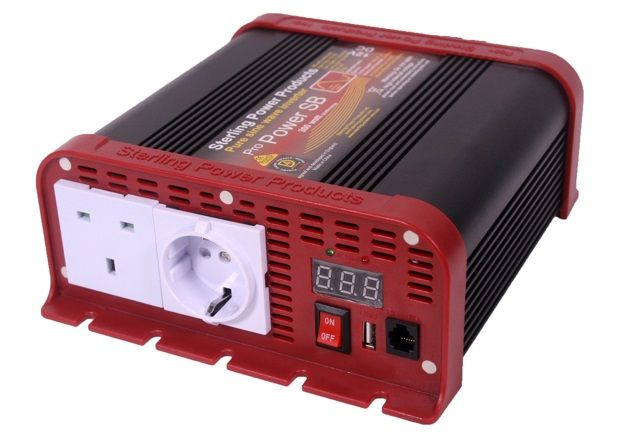
\includegraphics[width=0.15\paperwidth]{../Images/image_10_1_(inverter).png}
    \end{center}
    
    The component we need to do this is called an inverter. Inverters can be found relatively cheaply and easily. However, when choosing an inverter it is particularly important to remember that you get what you pay for.

    Unbranded cheap inverters have a number of drawbacks. Firstly, they can be very inefficient, wasting 20-30\% of the power supplied. This means your 60W laptop may consume more like 85W if powered through an inverter instead of through a 12V adapter.

    Secondly, cheap inverters produce a ‘modified’ sine wave that is not as smooth as that supplied by the national grid. The modified sine wave will contain noise which can affect the operation of certain appliances. Most audio equipment and some microwaves, printers, motors, power tools and computers will not work reliably with a modified sine wave inverter.

    Thirdly, cheap inverters are prone to burning out when subject to prolonged use. If you are building a system that is likely to be used continuously, it is worth choosing a reliable inverter from a reputable manufacturer, that will likely be more cost effective in the long run.

    Pure sine wave inverters can be a better choice than modified sine wave inverters, but will be more expensive. Pure sine wave inverters produce a sine wave that is as smooth as the national grid, meaning any appliance through them will work exactly as expected. They can also be more efficient in the power conversion, but this varies from inverter to inverter so do some research before buying.

    \begin{center}
      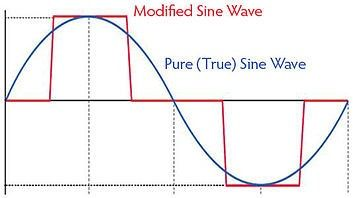
\includegraphics[width=0.30\paperwidth]{Images/image_10_2_(sine_wave).png}
    \end{center}
  
  % subsection inverters (end)

% section appliances (end)

{\color{blue}\section{Constructing a Simple 12V Off-Grid Circuit}} % (fold)
\label{sec:constructing_a_simple_12v_off_grid_circuit}

  The 'Circuit Diagram' shown below gives an overview of how to connect a solar panel, charge controller, battery, battery guard, fuse, lights, laptop charger and phone charger all together into a simple off grid circuit. 

  Note that there is no 'Load' connection (with the light bulb symbol) on the charge controller. This circuit assumes that a basic charge controller is used, so to provide suitable discharge control the load is connected directly to the battery via a battery guard. If using a charge controller with adequate current rating and low-voltage protection, you can assume that all ‘Load’ connections to the battery guard would be connected to the ‘Load’ terminals of the charge controller.

  Remember that a fuse connects only to the positive wire of the circuit and does not have a polarity.

  Note that the LED bulbs used in the 12V Off Grid workshop do not have a polarity to the user, as the internal circuitry within the bulbs can work both ways. This is not true of all LED lights so be sure to check, as you should do for all equipment when connecting DC electrical circuits.

  This circuit includes a multimeter to measure current on the load - this is for testing the circuit during the workshop demonstration, and is not essential, although in any off grid installation we would recommend having something in place to measure consumption.

  \begin{center}
    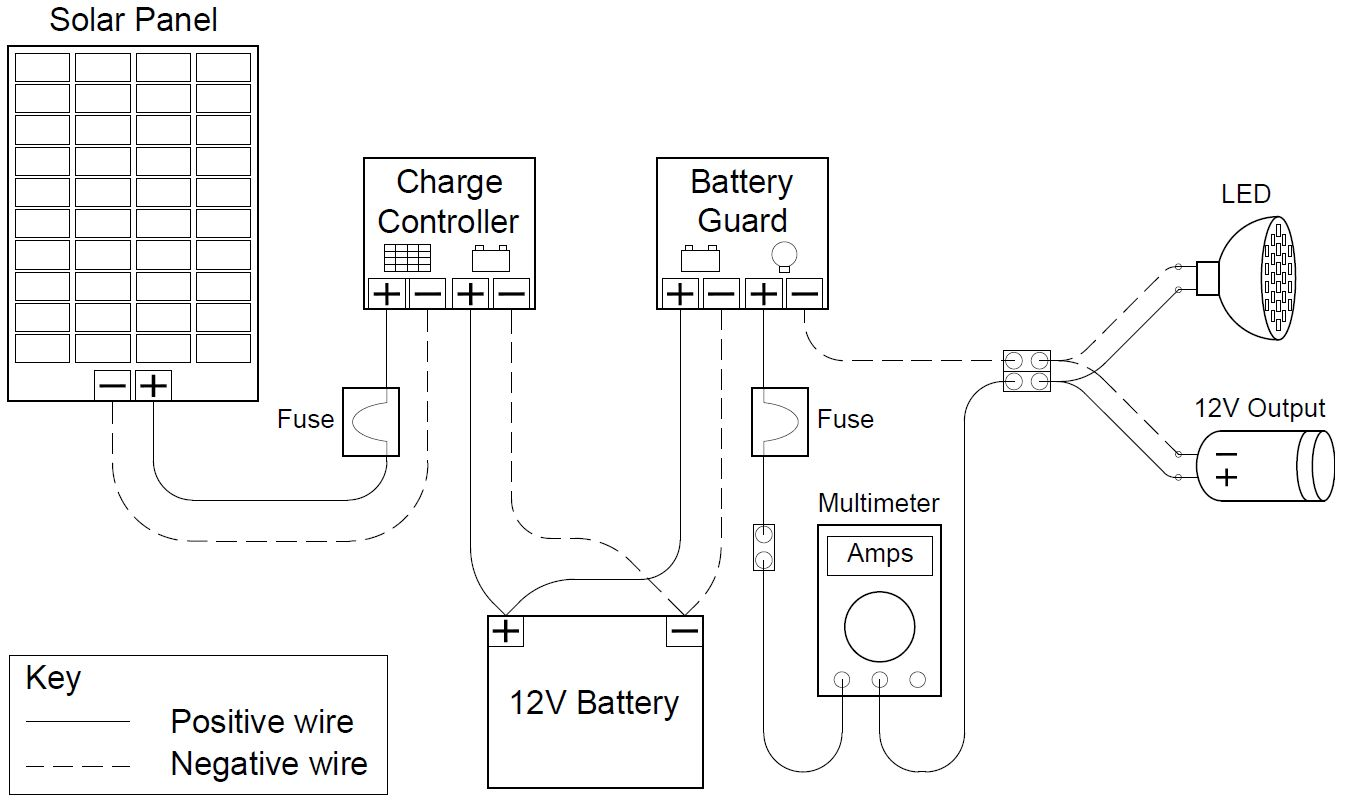
\includegraphics[width=0.75\paperwidth]{Images/image_11_2_(12v_system).png}
  \end{center}

  {\color{blue}\subsection{Basic system modelling}} % (fold)
  \label{sec:basic_system_modelling}
  
  % subsection basic_system_modelling (end)

  {\color{blue}\subsection{Designing an efficient system}} % (fold)
  \label{sub:designing_an_efficient_system}

    The key to designing an efficient off-grid electrical system is consideration of the power conversions used to run the appliances we wish to use. In modern conventional society we expect electricity to be abundant, meaning that its use as a general energy source can be taken for granted. In a solar off-grid system, particularly in the winter, electricity is not so freely available and thus ensuring that we use the right power supply for the right task is crucial. 

    As a general rule, for tasks needing electricity specifically, e.g. for lighting and charging devices, then the off-grid system is a good choice for power. For tasks needing mechanical or heat energy think about exploring alternative power sources.

    \subsubsection{Converting to heat} % (fold)
    \label{ssub:converting_to_heat}

      Conversion of electricity to heat is extremely power-intensive, particularly when you consider that most electricity was converted from inefficiently burning coal or gas in the first place. So things like a kettle, cooker, water or space heater could easily push the specifications of your system into an unaffordable or impractical range. Consider using efficient fuel-burning sources for heating water and cooking. Raising the temperature of water by a few degrees before heating or boiling can also dramatically cut down on power consumption. Consider ground source heat, biomass heat and solar thermal instead of electrical heating. Insulation is also key, as an uninsulated boiler or house will balance temperature with the external temperature all too readily. 
    
    % subsubsection converting_to_heat (end)

    \subsubsection{Converting to cold} % (fold)
    \label{ssub:converting_to_cold}

      Fridges and freezers are a mid-high consumer of household power, mainly because they are always on. When designing your system consider if your freezer is really necessary. In the UK fridges are only actually significantly cooler than the outside temperature for a few short months of the year. And conveniently these months correlate to when there is the most energy available from the sun. Consider if you can have a cool box outside in the winter months to reduce your refrigeration requirements while the sun isn't shining. 
    
    % subsubsection converting_to_cold (end)

    \subsubsection{Converting to mechanical} % (fold)
    \label{ssub:converting_to_mechanical}

      Conversion of electricity to mechanical energy is more efficient than heat, but it is worth considering if any conversion is required at all. Consider hand powered juicers, blenders and smoothie makers. Bicycle powered designs are fun for children but require some knowledge of mechanics and metalwork. Cycle powered washing machines exist, but many that build them revert to using electrical systems as a time saving measure. The main energy requirement in washing is heating the water, so electrical washing machines are not overly inefficient as long as you wash with cold water or use an alternative power source to heat the water first. 
    
    % subsubsection converting_to_mechanical (end)

    \subsubsection{Inverting to 240AC} % (fold)
    \label{ssub:inverting_to_240ac}

      As explored in the section on Inverters, inverting to 240AC can be extremely inefficient. Sometimes it is necessary to invert but in an off-grid system it can be a good idea to minimise the amount of electricity you need to invert. Consider what you really need to invert for. Can any of this be done in a different way? In a solar powered system you will likely have excess electricity in the summertime so appliances that you will use more in the summertime may well not be an issue.
    
    % subsubsection inverting_to_240ac (end)
  
  % subsection designing_an_efficient_system (end)

  {\color{blue}\subsection{Planning Your System}} % (fold)
  \label{sub:planning_your_system}

    Planning an off-grid system will generally be a series of trade-offs. Perhaps you have a limited number of panels and wish to figure out how many batteries to invest in. Or perhaps you are able to aquire a large number of panels and wish to minimise the number of batteries in your system. There will always be a trade off between consumption, generation (from panels) and storage (in batteries). 

    Planning an off grid system generally involves starting at the end (consumption) and working your way backwards towards the start (generation). You should always consider the worst case scenario when planning your system - a day when all your appliances are going to be in use, with the least amount of generation coming in.
  
  % subsection planning_your_system (end)

  {\color{blue}\subsection{Calculating your consumption}} % (fold)
  \label{sub:calculating_your_consumption}

    In order to plan your off grid system you need to start by considering what you actually wish to power. Find the power consumption of the appliances you wish to include by looking at their specifications, which will either be printed on an appliance or will be in its manual. Power consumption will be indicated in watts (W) or kilowatts (kW). Sometimes the appliance will indicate the current draw in Amps (A), which will need to be multiplied by the voltage of the appliance to calculate the power consumption in watts.

    Power values on appliances may be estimates, or may represent the maximum consumption on an appliance with variable power levels. For an accurate measurement of how much power an appliance consumes under actual usage conditions, you can use a plug-in power monitor that records power consumed over time. 

    \begin{center}
      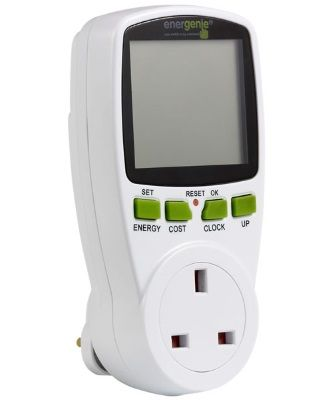
\includegraphics[width=0.15\paperwidth]{../Images/image_12_1_(watt_meter).png}
    \end{center}

    Examples: 

    TODO ADD EQUATION

    Next, think about how many hours you might wish to power your appliance per day. This will give you the energy consumption of the appliance, a measure of power over time. Note that this might be different between summer and winter. See section 'Considerations – Summer to Winter' for more details about comparing summer to winter.

    Examples:

    TODO ADD EQUATION

    Any appliances that run off an AC power supply will need to factor in the efficiency of the inverter being used, since there will be energy lost in the conversion from DC to AC. See the ‘System losses’ section below for more details.

    Now you will be able to calculate your total daily power consumption.
    
    TODO ADD EQUATION
  
  % subsection calculating_your_consumption (end)

  {\color{blue}\subsection{Calculating battery storage}} % (fold)
  \label{sub:calculating_battery_storage}

    The easiest way to size your battery storage is to consider times of the year where there will be little to no solar generation coming in. At these times, you batteries will need to store enough energy to match your consumption over those days, without being discharged too low.

    In the UK, it is recommended to plan for 3 days worth of storage for your battery bank. To calculate the total energy storage of your battery bank, you will need to multiply your daily consumption by 3, then double it to ensure your batteries stay above 50\% S.o.C. after 3 days use.

    TODO ADD EQUATION

    To calculate the battery capacity needed in Amp hours (Ah), we need to divide the energy storage by the voltage of the batteries being used, using the relationship between power, volts and amps. So if using 12V batteries, divide the Wh by 12.

    TODO ADD EQUATION

    Our battery bank capacity will need to accommodate 770 Amp Hours. This is a conservative figure, using the worst case scenario, so there will be very few times when this storage will be required, but by conservatively sizing your battery bank you can be confident that they will last as long as possible.

    This is not an unrealistic battery bank, using large 100-200 Amp Hour batteries connected in parallel. However given the expense of large batteries it may not be something you can do right away, but rather a system that you build up to.

  % subsection calculating_battery_storage (end)

  {\color{blue}\subsection{Calculating solar generation}} % (fold)
  \label{sub:calculating_solar_generation}

    Now that we know our daily power consumption, we can calculate the power we can generate from our solar panels.

    Crucially, the power rating of a solar panel does not mean that the panel will generate that power every hour that the sun is out. In the UK, as a rule of thumb, the panel will generate 4.5 hours equivalent peak in summer and 1 hour equivalent peak in winter. This means a 100W panel will produce 450Wh per day in summer and 100Wh per day in winter. Very good online calculators exist to assist with this over the course of the year. We use this calculator:

    Europe: \href{http://re.jrc.ec.europa.eu/pvgis/apps4/pvest.php?lang=en\&map=europe}{\underline{http://re.jrc.ec.europa.eu/pvgis/apps4/pvest.php?lang=en\&map=europe}}

    Africa: \href{http://re.jrc.ec.europa.eu/pvgis/apps4/pvest.php?map=africa\&lang=en}{\underline{http://re.jrc.ec.europa.eu/pvgis/apps4/pvest.php?map=africa\&lang=en}}

    Using the European calculator to estimate optimum generation from a 1kW crystalline silicon system in Bristol without including any system losses from cables or internal components we see the following energy generation on a daily and monthly basis.

    TODO ADD TABLE

    As a general rule, average daily generation should match average daily consumption. So to generate 1.535kWh of energy per day in December, we would need around 1.4kW of solar panels (1.535 / 1.11). This would mean we will generate far more than we use in summer, but would ensure that we don’t suffer a shortfall in winter. To avoid over-producing generation in summer, you can consider ways to reduce consumption in winter and increase it in summer, and size your solar generation according to spring/autumn values.
  
  % subsection calculating_solar_generation (end)

  {\color{blue}\subsection{System losses}} % (fold)
  \label{sub:system_losses}

    When doing all these calculations, you need to take into account any energy losses within the system. These losses come from internal wire resistance, inversion and conversion losses, and losses through your charge controller. For a detailed design you should check the specifications of each component you wish to use in your system, make a note of its efficiency rating, and adjust power generation and consumption calculations as appropriate. For a basic design you can assume overall system losses of 15\%.

    Charge controllers will reduce the energy being generated from the solar panels by 20-30\% for PWM controllers and 5\% for MPPT controllers. 

    Inverters will increase the power consumed by AC appliances being run through them relative to their efficiency, e.g. a 500W appliance being powered through an inverter with an efficiency of 90\% will draw 500 \(\div\) 0.9 = 555W.

    Step up and step down DC converters will lose energy in conversion, and basic ones may have an efficiency as low as 60\%, but better models are more likely to be around 80-85\%. 

    For small systems with adequate wire sizes, transmission losses should not be above 3\%.  
  
  % subsection system_losses (end)

% section constructing_a_simple_12v_off_grid_circuit (end)

{\color{blue}\section{Additional system modelling}} % (fold)
\label{sec:additional_system_modelling}

  {\color{blue}\subsection{Balancing seasonal generation with battery storage}} % (fold)
  \label{sub:balancing_seasonal_generation_with_battery_storage}

    In higher latitudes one of the most crucial aspects when considering the capacity of your battery bank is the difference in power generation between summer and winter. For a perfectly utilized system, if we are to rely on solar as our renewable energy source, we will either need to use much less power in winter or we will need to store energy generated in summer to be used in winter. Realistically we will probably need to do a combination by having some battery storage AND reducing our demands in winter.

    Looking at the yearly average of the 1kW Bristolian system outlined above we can see that potentially we could use almost 3 kWh per day, on average through the year. So we can calculate the size of solar array needed for an average daily consumption of 1535 Wh:

    TODO ADD EQUATION

    So a solar array with a combined peak power rating of 520 Watts will generate 1535 Wh per day on average throughout the year. We can use the PVGIS calculator to work out how much an array of this size would generate per month.

    To calculate how much battery storage we need, we would start by calculating the deficit through the winter from our 1535 Wh per day usage. Note that we could similarly calculate the summer surplus and get the same result.

    We find a deficit in October through to February:

    TODO ADD EQUATION

    So our battery bank will need to store at least this much if we wish to use our yearly average every day. We will need to store twice this much (6900 Wh) if we wish to prevent our batteries discharging below 50\% S.o.C. Working with 12V batteries we can convert our total deficit amount to Amp hours as before to calculate the battery capacity needed.

    TODO ADD EQUATION

    The seasonal balancing method results in smaller solar array and a somewhat smaller battery bank than the basic method described above, but it is worth thinking about the assumptions made to reach that result. Effective seasonal storage relies on consistent average energy generation and consumption through the winter - if there are a couple of days where generation is lower than expected and/or consumption is higher than expected, you will find your batteries are discharged lower than planned. 

    It is generally worth having too much capacity in your system (i.e. slightly more generation and battery storage than you actually need) than too little capacity. This will help mitigate an exceptionally cold, wet and cloudy period in which you generate less than expected. 
  
  % subsection balancing_seasonal_generation_with_battery_storage (end)

  {\color{blue}\subsection{Time of day consumption modelling}} % (fold)
  \label{sub:time_of_day_consumption_modelling}

    One of the major considerations in designing a renewable power systems is the accessibility of power when the renewables are not generating.

    The difference between day and night energy usage can be a big consideration in optimising an off grid system, especially in parts of the world closer to the equator. With a smaller difference in generation between seasons the whole system can be much more easily optimised, focussing around generating enough in the day to sustain power usage at night.

    Shifting time of day consumption to match generation from the solar panels reduces the need to store energy for use at night. In the example used previously, the fridge is running continuously for 24 hours, but on average 12 of those hours will be in daylight when the solar panels are generating. We can also assume that the laptop will be charged during daylight hours. That reduces the energy storage value by 420 Wh, almost a third of the original size. 

    When calculating energy consumption, make an estimate of when each appliance will be used, and any consumption taking place during the middle of the day (8am - 4pm) can be discounted from the total when working out energy storage.
  
  % subsection time_of_day_consumption_modelling (end)

  {\color{blue}\subsection{Where to compromise}} % (fold)
  \label{sub:where_to_compromise}

    When planning and designing your system you will generally have one of two priorities, either to make a system within budget, or to have enough power to meet all your needs.

    If building a system to budget is your primary concern start by working out your budget. 

    The main costs to consider are:

    \begin{enumerate}
      \item Batteries: Find a source of leisure or deep cycle batteries (ask around and you will find a second hand source). A good price might be around £1 per 4Ah.
      \item Panels: If DIY then you can build a small array for as little as 40p/W with enough time and patience, but you can also buy second hand panels for around the same price.
      \item Charge Controller: £10 up to 200W system (depending on panels), £50 for cheap MPPT, for systems over 400W consider investing more in you charge controller.
      \item For a small system with less than 200W of solar, it is not worth spending extra for an MPPT charge controller, but for systems over 800W it is almost certainly worth it.
      \item The more appliances you can run directly from DC power, the better, but you shouldn’t go out and buy replacements for all your existing appliances just to avoid using AC power.
      \item If you are expecting to use a lot of AC appliances, it is worth spending more for a good quality inverter that will work reliably for longer.
    \end{enumerate}

    In all cases, you want to make sure that you are as accurate as possible with your energy consumption estimates, since - while you want to avoid spending more than you need to - a system that is under-capacity will run into problems when solar generation starts to fall off in winter.

    By taking an iterative approach to system design, you can find the right compromise between system capacity and budget. Just follow the following process as many times as you want:

    \begin{enumerate}
      \item Calculating Your Power Consumption: You can do this either month by month, for summer and winter, or just a flat consumption all year. You can also take daytime consumption into account.
      \item Calculate Power from Panels: From this you should be able to gauge the approximate size of the solar array needed, using your total yearly requirements and then finding an array that will generate this using the online calculators outlined above. This will give you the minimum number of panels required, a good baseline to begin with. 
      \item Calculating Required Battery Storage: Now calculate the months in which you will have a surplus and those in which you will have a deficit of power. You'll need to ensure that you have a battery bank with capacity to store the excess power across all consecutive months of deficit. You should also have a battery bank that can store at least two days worth of energy consumption from your most essential appliances.
      \item Once you have calculated the size of your battery bank, consider if it makes economic or practical sense to have a battery bank and solar array of this size. If so, great, you have a plan. If not repeat the process by cutting back on consumption, and adjusting the number of panels and batteries accordingly.
    \end{enumerate}

    For example, in our previous case study, we could reduce the power consumption by using an outdoor cool box instead of a fridge in winter, and by using a stove powered by wood or gas to boil water instead of an electric kettle. Since these are the two largest sources of energy consumption in our system, this would drastically reduce the size of generation and storage needed.
  
  % subsection where_to_compromise (end)

% section additional_system_modelling (end)

{\color{blue}\section{Constructing the Whole System}} % (fold)
\label{sec:constructing_the_whole_system}

  In constructing your whole system there are a few important questions to consider:

  \textbf{Am I going to need to transport power over distances long enough to warrant stepping up the voltage?}

  If you answered 'yes' you should consider connecting the batteries in your battery bank in series, to increase the voltage. Once you have chosen your system voltage (12V, 24V or 48V), you may need to add ‘strings’ of batteries in parallel, to increase the capacity of the battery bank. You will then be able to transport your electricity at the 'stepped up' voltage and just use a step down at the usage end to take it back to 12V. If you don't need to step up your voltage for transmission you will generally be happy with a 12V battery bank, connecting all batteries in parallel.

  \begin{center}
    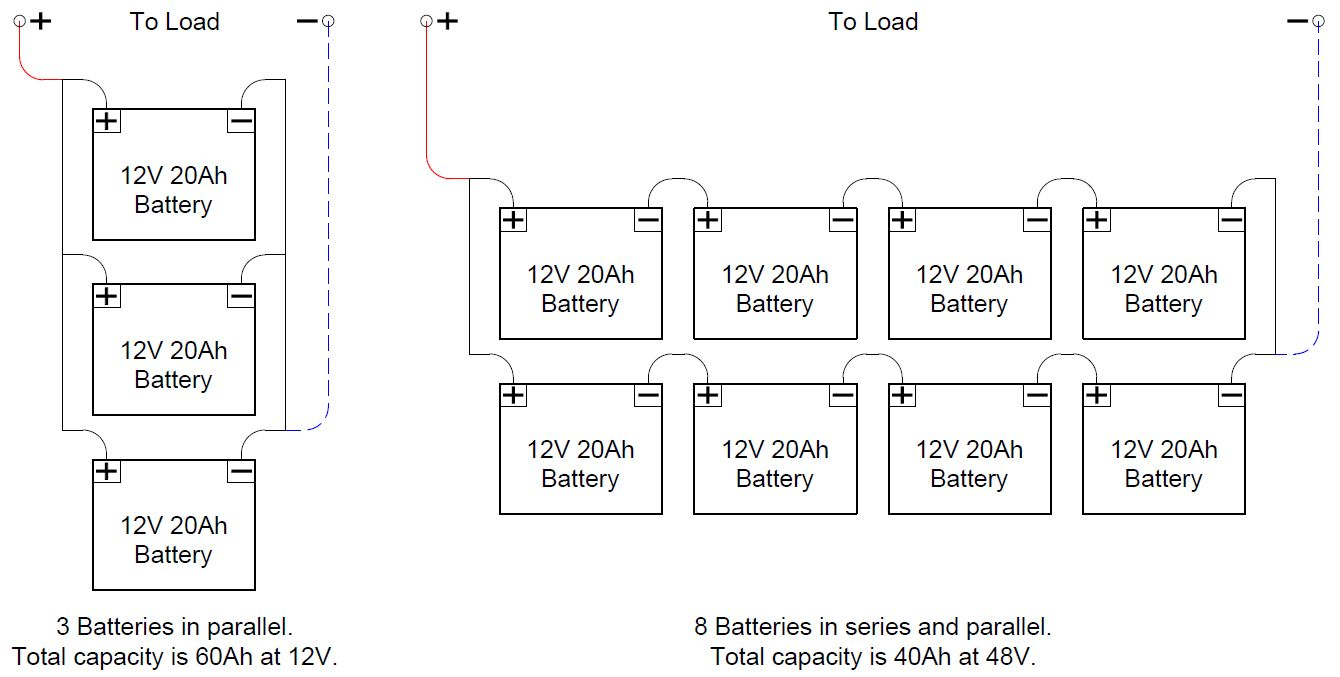
\includegraphics[width=0.75\paperwidth]{Images/image_13_1_(whole_system_1).png}
  \end{center}

  When assembling a battery bank, make sure that all batteries you use are as identical as possible - use the same make and model of battery, and don’t mix new and old batteries in the same battery bank. You should also try to use the thickest, most heavy duty cables for connecting batteries together. This is because any internal resistance in the battery bank can cause the amount of charging and discharging individual batteries are exposed to become unbalanced, which can cause over-worked batteries to fail much sooner. Make sure to regularly isolate each string of batteries in parallel, and check their voltage to make sure they are all working as expected. 

  \textbf{What voltage/current can my charge controller handle?}

  The answer to this question will indicate how you connect together your panels. You may wish to connect all of your panels together in series to increase voltage and lower resistive losses. However, when dealing with multiple panels you will need to be sure your charge controller can handle this. For example, let’s assume we are using a basic charge controller rated for a current of 20A and a voltage of 50V, and 4x200W panels rated at 10A peak current and an open-circuit voltage of 20V. We have to make sure our solar array doesn’t generate above those values, by planning how we connect them together.
  
  \begin{center}
    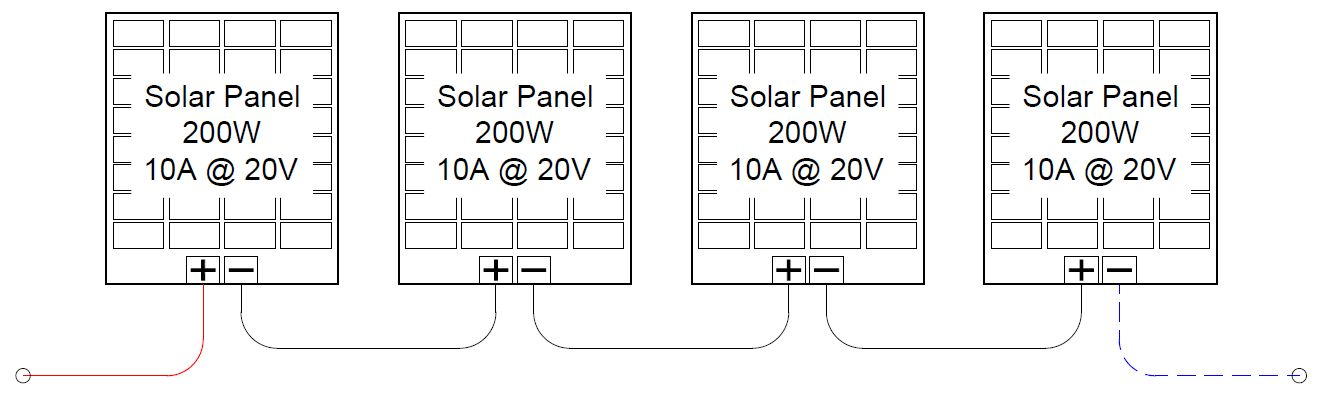
\includegraphics[width=0.75\paperwidth]{Images/image_13_2_(whole_system_2).png}
  \end{center}
  
  Connecting 4 panels in series: Each panel is rated at 10A @ 20V so total output would be 2A @ 80V.

  \begin{center}
    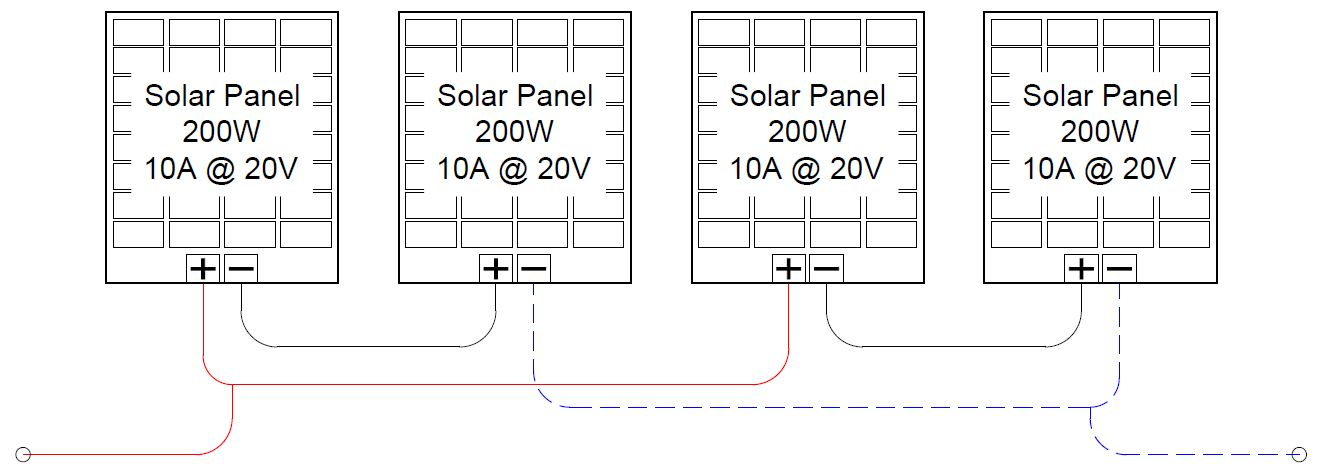
\includegraphics[width=0.75\paperwidth]{Images/image_13_3_(whole_system_3).png}
  \end{center}

  Connecting 4 panels in series and parallel. Each panel is rated at 10A @ 20V so total output would be 20A @ 40V. This would be the configuration we would need to use with our example charge controller, since the first arrangement would generate above 50V, which would damage the charge controller.

  You will also need to ensure the charge controller can accommodate the voltage of your battery bank. Most charge controllers will work automatically with either 12V or 24V systems without any trouble but be sure to check the specifications of whatever charge controller you choose to use.

  If using a PWM charge controller, you should plan the open circuit voltage of your solar array to be around 18V for a 12V battery bank, and 36V for a 24V battery bank. PWM charge controllers can accept higher voltages, but the higher the voltage, the bigger the generation losses will be, because PWM charge controllers do not regulate voltage efficiently. MPPT charge controllers are able to convert voltages without losing nearly as much energy, so they make having a solar array with a higher voltage than the battery bank much more viable.

% section constructing_the_whole_system (end)

{\color{blue}\section{Resources}} % (fold)
\label{sec:resources}

  \subsubsection{Useful Information for Installations} % (fold)
  \label{ssub:useful_information_for_installations}

    \begin{enumerate}
      \item How a lead acid battery works: \href{http://www.progressivedyn.com/battery\_basics.html}{\underline{http://www.progressivedyn.com/battery\_basics.html}}
      \item How a MPPT charge controller works: \newline
      \href{http://en.wikipedia.org/wiki/Maximum\_power\_point\_tracking}{\underline{http://en.wikipedia.org/wiki/Maximum\_power\_point\_tracking}}
      \item Calculating line losses: A handy calculator to help you work out losses over distance for different \newline
      thickness of wire. \href{http://www.solar-wind.co.uk/cable-sizing-DC-cables.html}{\underline{http://www.solar-wind.co.uk/cable-sizing-DC-cables.html}}
      \item Calculate PV generation throughout the year. \newline
      Europe: \href{http://re.jrc.ec.europa.eu/pvgis/apps4/pvest.php?lang=en\&map=europe}{\underline{http://re.jrc.ec.europa.eu/pvgis/apps4/pvest.php?lang=en\&map=europe}} \newline
      Africa: \href{http://re.jrc.ec.europa.eu/pvgis/apps4/pvest.php?map=africa\&lang=en}{\underline{http://re.jrc.ec.europa.eu/pvgis/apps4/pvest.php?map=africa\&lang=en}}
    \end{enumerate}
  
  % subsubsection useful_information_for_installations (end)

  \subsubsection{Other Renewable Energy Resources} % (fold)
  \label{ssub:other_renewable_energy_resources}
  
    \begin{enumerate}[resume]
      \item DIY solar panels: \href{https://www.demandenergyequality.org/build-your-own-panels}{\underline{https://www.demandenergyequality.org/build-your-own-panels}}
      \item How solar cells work: \href{https://www.demandenergyequality.org/guide-to-solar-energy}{\underline{https://www.demandenergyequality.org/guide-to-solar-energy}}
      \item DIY wind turbines: \newline
      V3 Power run courses: \href{http://v3power.co.uk/}{\underline{http://v3power.co.uk/}} \newline
      Hugh Piggott Designs: \href{http://scoraigwind.co.uk/}{\underline{http://scoraigwind.co.uk/}}
      \item DIY micro hydro at Steward Wood Community: \newline
      \href{http://www.stewardwood.org/resources/hydroelectric.ghtml}{\underline{http://www.stewardwood.org/resources/hydroelectric.ghtml}} \newline
      \href{https://www.permaculture.co.uk/articles/310505923/building-your-own-renewable-energy-systems-recycled-materials}{\underline{https://www.permaculture.co.uk/articles/310505923/building-your-own-renewable-energy-systems-recycled-materials}}
      \item Cycle powered generation: \href{http://www.stewardwood.org/resources/DIYcyclepower.htm}{\underline{http://www.stewardwood.org/resources/DIYcyclepower.htm}}
      \item Renewable energy diagram by Merlin Howse: \newline
      \href{http://offthegrid.org.uk/resources/renewable-energy-diagram-2.0.pdf}{\underline{http://offthegrid.org.uk/resources/renewable-energy-diagram-2.0.pdf}}
    \end{enumerate}


  % subsubsection other_renewable_energy_resources (end)

  \subsubsection{Off grid system component suppliers} % (fold)
  \label{ssub:off_grid_system_component_suppliers}

    \begin{enumerate}[resume]
      \item Wind and Sun: \href{http://www.windandsun.co.uk/}{\underline{http://www.windandsun.co.uk/}}
      \item Bimble Solar: \href{http://www.bimblesolar.com/}{\underline{http://www.bimblesolar.com/}}
    \end{enumerate}
  
  % subsubsection off_grid_system_component_suppliers (end)

% section resources (end)

{\color{blue}\section{Appendices}} % (fold)
\label{sec:appendices}

  {\color{blue}\subsection{Equipment List}} % (fold)
  \label{sub:equipment_list}

    \textbf{Equipment – System Level} \newline
    Batteries \newline
    Solar panels or renewable energy source \newline
    Charge controller \newline
    Battery guard \newline
    Fuses \newline
    Wire \newline
    DC voltage step-ups and step-downs \newline
    System monitor

    \textbf{Equipment – Usage Level} \newline
    Connectors eg terminal blocks, crimp \newline
    connectors, lugs, MC4, XT60, Anderson \newline
    DC Switches \newline
    Cigarette lighter socket \newline
    12V to USB converter \newline
    12V laptop charger \newline
    12V LEDs \newline
    Inverter

    \textbf{Equipment – Tools} \newline
    Multimeter \newline
    Wire strippers \newline
    Wire cutters \newline
    Screwdrivers \newline
    Spanners \newline
    Crimping tool \newline
    A connector clamp \newline
    A load tester (for testing batteries) \newline
    Soldering iron + solder
      
  % subsection equipment_list (end)

  {\color{blue}\subsection{Using a Multimeter}} % (fold)
  \label{sub:using_a_multimeter}

    \begin{figure}[!ht]
      \centering
      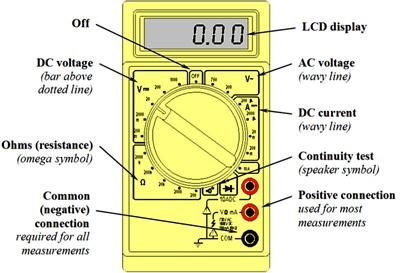
\includegraphics[width=0.65\paperwidth]{Images/image_a_1_(multimeter).png}
      \caption*{Image from 500tips.com}
    \end{figure}
  
  % subsection using_a_multimeter (end)

% section appendices (end)

\end{document}